\documentclass{article}
\usepackage[utf8]{inputenc}
\usepackage[russian]{babel}
\usepackage[left=2cm,right=2cm,
top=2cm,bottom=2cm,bindingoffset=0cm]{geometry}
\usepackage{graphicx}
\usepackage{amsmath}
\usepackage{float}
\usepackage{listings}
\usepackage{url,textcomp}
\date{2019 г.}
\author{Кондратенко Федор, гр 13632/1}
\setlength{\parindent}{0pt}
\setlength{\parskip}{5pt plus 2pt minus 1pt}
\frenchspacing
\title{Отчет по заданию №4.2}
\lstset{
	literate={а}{{\selectfont\char224}}1
	{б}{{\selectfont\char225}}1
	{в}{{\selectfont\char226}}1
	{г}{{\selectfont\char227}}1
	{д}{{\selectfont\char228}}1
	{е}{{\selectfont\char229}}1
	{ё}{{\"e}}1
	{ж}{{\selectfont\char230}}1
	{з}{{\selectfont\char231}}1
	{и}{{\selectfont\char232}}1
	{й}{{\selectfont\char233}}1
	{к}{{\selectfont\char234}}1
	{л}{{\selectfont\char235}}1
	{м}{{\selectfont\char236}}1
	{н}{{\selectfont\char237}}1
	{о}{{\selectfont\char238}}1
	{п}{{\selectfont\char239}}1
	{р}{{\selectfont\char240}}1
	{с}{{\selectfont\char241}}1
	{т}{{\selectfont\char242}}1
	{у}{{\selectfont\char243}}1
	{ф}{{\selectfont\char244}}1
	{х}{{\selectfont\char245}}1
	{ц}{{\selectfont\char246}}1
	{ч}{{\selectfont\char247}}1
	{ш}{{\selectfont\char248}}1
	{щ}{{\selectfont\char249}}1
	{ъ}{{\selectfont\char250}}1
	{ы}{{\selectfont\char251}}1
	{ь}{{\selectfont\char252}}1
	{э}{{\selectfont\char253}}1
	{ю}{{\selectfont\char254}}1
	{я}{{\selectfont\char255}}1
	{А}{{\selectfont\char192}}1
	{Б}{{\selectfont\char193}}1
	{В}{{\selectfont\char194}}1
	{Г}{{\selectfont\char195}}1
	{Д}{{\selectfont\char196}}1
	{Е}{{\selectfont\char197}}1
	{Ё}{{\"E}}1
	{Ж}{{\selectfont\char198}}1
	{З}{{\selectfont\char199}}1
	{И}{{\selectfont\char200}}1
	{Й}{{\selectfont\char201}}1
	{К}{{\selectfont\char202}}1
	{Л}{{\selectfont\char203}}1
	{М}{{\selectfont\char204}}1
	{Н}{{\selectfont\char205}}1
	{О}{{\selectfont\char206}}1
	{П}{{\selectfont\char207}}1
	{Р}{{\selectfont\char208}}1
	{С}{{\selectfont\char209}}1
	{Т}{{\selectfont\char210}}1
	{У}{{\selectfont\char211}}1
	{Ф}{{\selectfont\char212}}1
	{Х}{{\selectfont\char213}}1
	{Ц}{{\selectfont\char214}}1
	{Ч}{{\selectfont\char215}}1
	{Ш}{{\selectfont\char216}}1
	{Щ}{{\selectfont\char217}}1
	{Ъ}{{\selectfont\char218}}1
	{Ы}{{\selectfont\char219}}1
	{Ь}{{\selectfont\char220}}1
	{Э}{{\selectfont\char221}}1
	{Ю}{{\selectfont\char222}}1
	{Я}{{\selectfont\char223}}1
}
\begin{document}
	\maketitle
	\section*{Создание пространства состояний}
	Для создания пространства состояний использовались следующие параметры:
	$$m_1 = 30,\ b_1 = 30,\ c_1 = 4650,\ m_2 = 3.6,\ b_2 = 10,\ c_2 = 400.$$
	Параметр $b_1$ был специально уменьшен, так как при исходном параметре $b^0_1=1200$ линейный анализ системы выполнить не удавалось.\\
	Были созданы матрицы A, B, C, D, используя следующий набор команд:
	\lstset{frameround=fttt}
	\begin{lstlisting}[firstnumber=1, frame=trBL, firstnumber=1,label=some-code,caption=Создание матриц для пространства состояний]]
	A = [0  1  0  0;
		-(c1 + c2)/m1  -(b1 + b2)/m1  c2/m1  b2/m1;
	  	0  0  0  1;
	  	c2/m2  b2/m2  -c2/m2  -b2/m2];
	B = [0 0; 1/m1 0; 0 0; 0 1/m2];
	C = eye(4);
	D = zeros(4, 2);
	\end{lstlisting}
	\section*{SSP Simulink}
	\paragraph*{Блок-схемы и моделирование}
	Была создана следующая блок-схема:
	\begin{figure}[H]
		\centering
		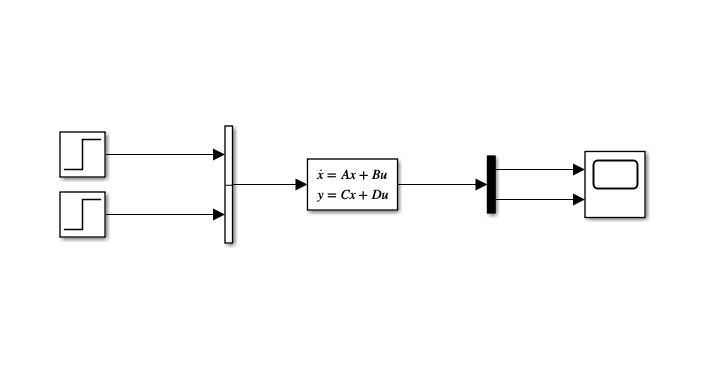
\includegraphics[width=0.7\linewidth]{sx_1}
		\caption{Блок-схема для получения Step-response}
		\label{fig:sx1}
	\end{figure}
	График реакции системы на Step-сигнал:
	\begin{figure}[H]
		\centering
		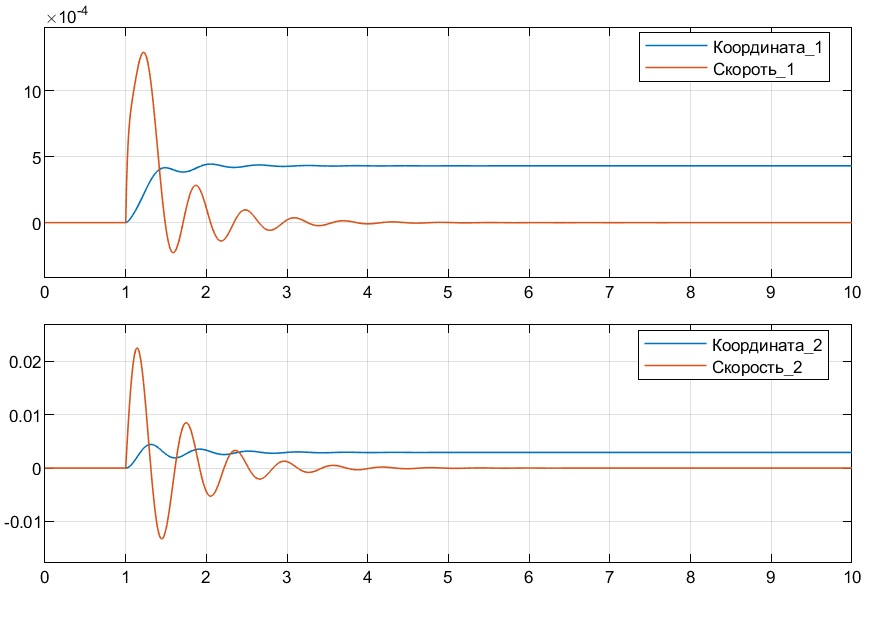
\includegraphics[width=0.7\linewidth]{sstep}
		\caption{Simulink Step-response}
		\label{fig:sstep}
	\end{figure}
	Далее Step-сигнал был заменен на Sine Wave:
	\begin{figure}[H]
		\centering
		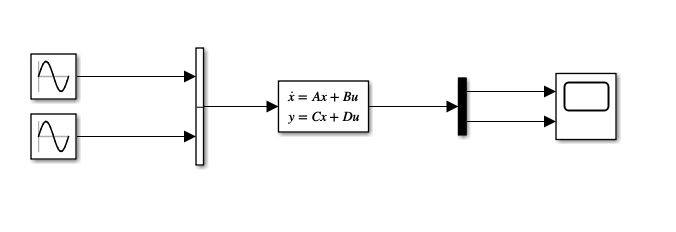
\includegraphics[width=0.7\linewidth]{sx2}
		\caption{Блок-схема для получения реакции на синусоидальный сигнал}
		\label{fig:sx2}
	\end{figure}
	График реакции системы:
	\begin{figure}[H]
		\centering
		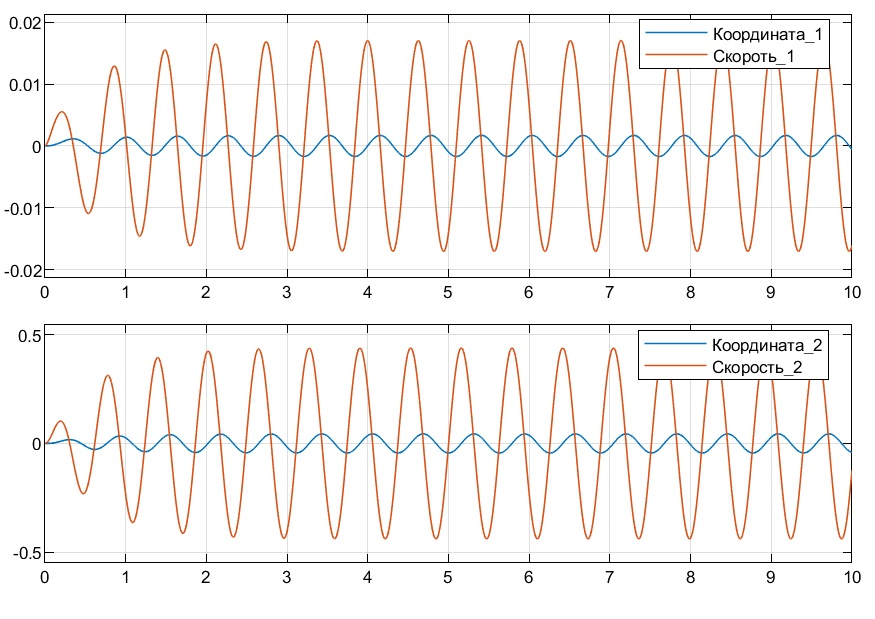
\includegraphics[width=0.7\linewidth]{ssine}
		\caption{$\omega = 10$, амплитуда $A = 5$}
		\label{fig:ssine}
	\end{figure}
	\paragraph*{Линейный анализ системы}
	Изначально линейный анализ проводился при $b^0_1=1200$, но на Singular Value plot не было видно второй резонансной частоты:
	\begin{figure}[H]
		\centering
		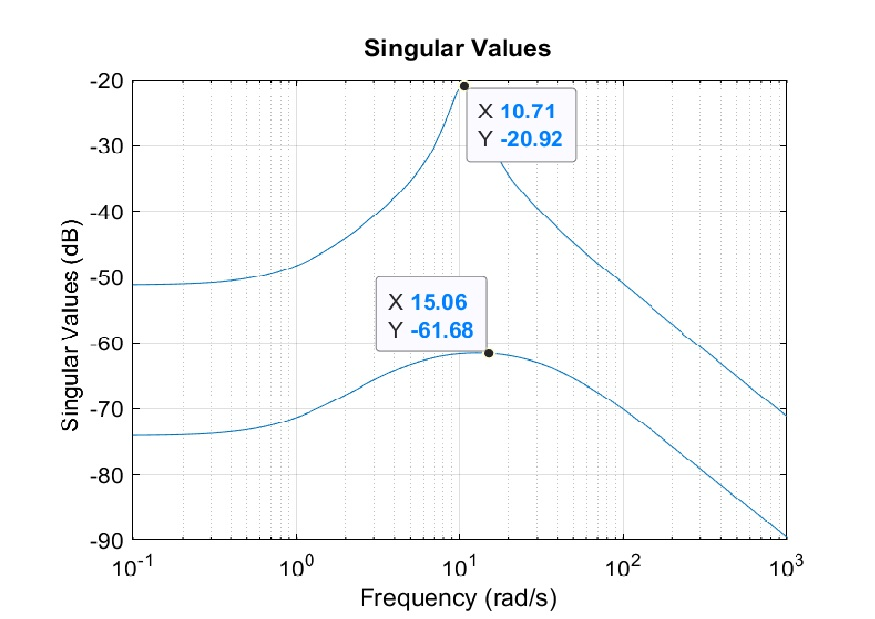
\includegraphics[width=0.7\linewidth]{sv1200}
		\caption{Singular Value plot, $b_1 = 1200$. Отчетливо видно отсутсвие второго максимума на графиках.}
		\label{fig:sv1200}
	\end{figure}
	Поэтому $b_1$ было уменьшено до 30:
	\begin{figure}[H]
		\centering
		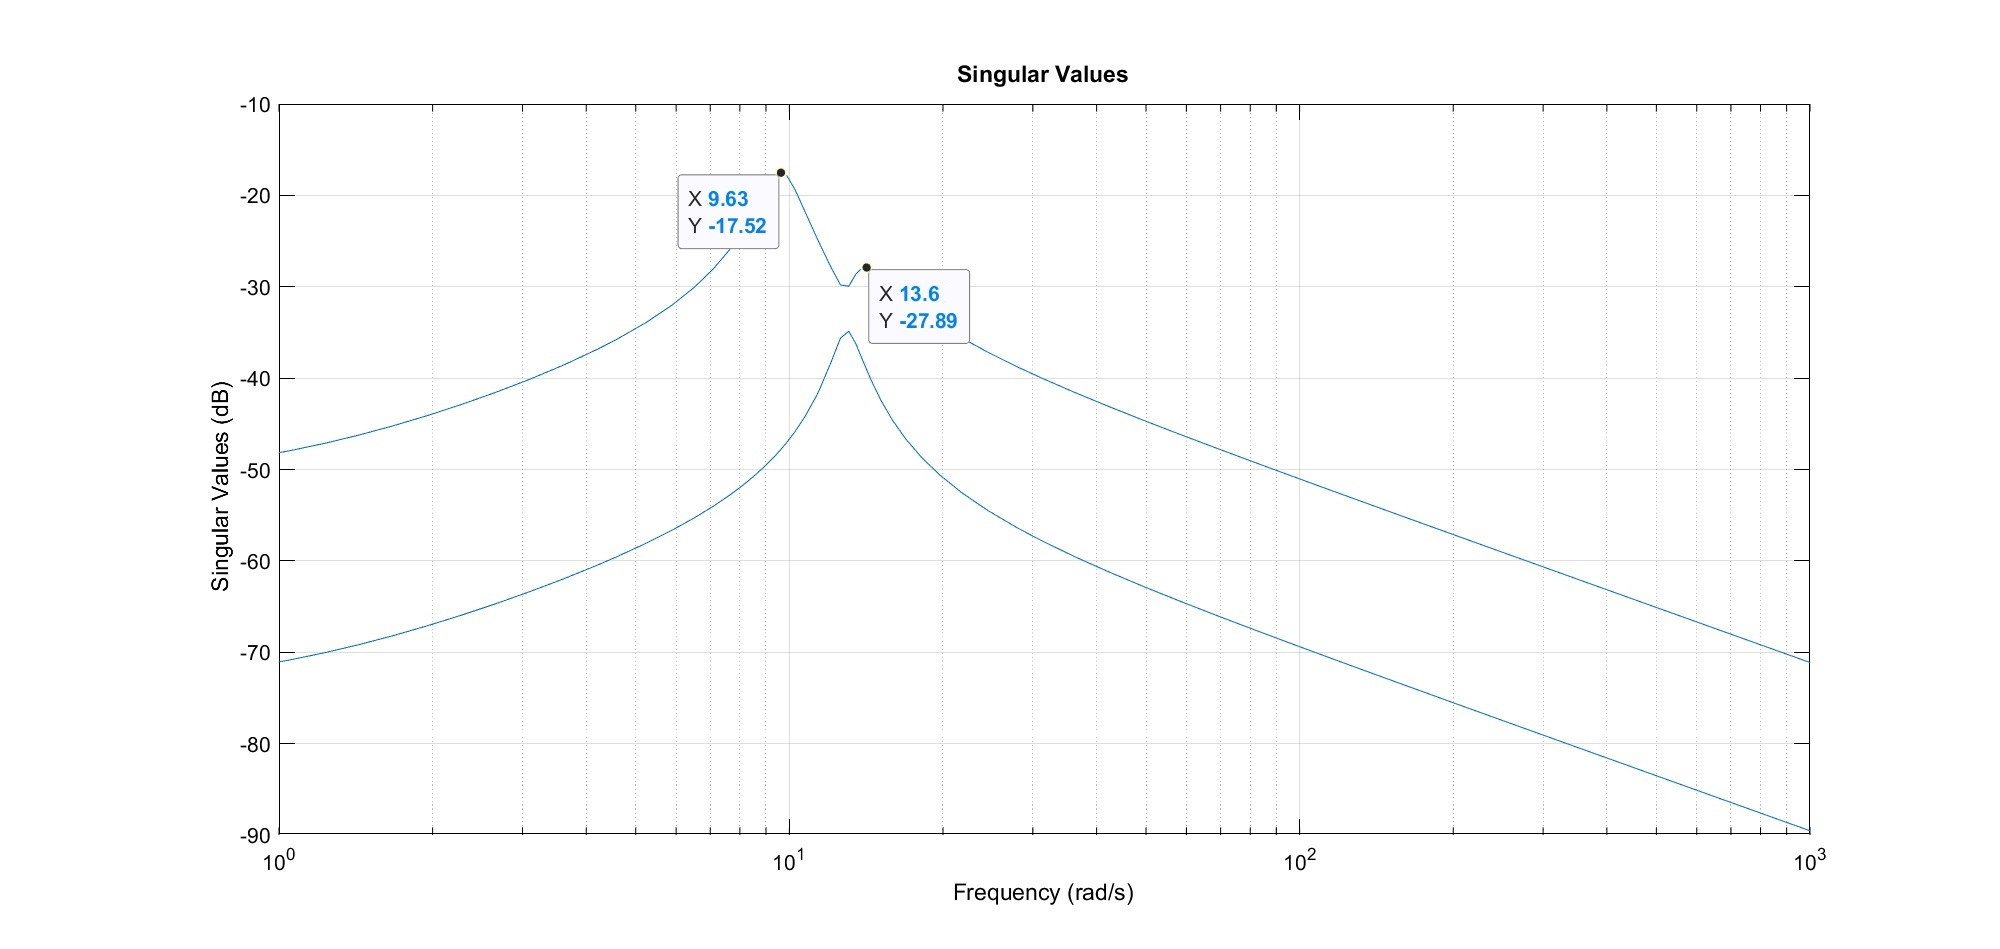
\includegraphics[width=0.7\linewidth]{sv30}
		\caption{Singular Value plot, $k_1 = 9.64,\ k_2 = 13.6$}
		\label{fig:sv30}
	\end{figure}
	С этим же значением $b_1$ был получен Bode Plot:
	\begin{figure}[H]
		\centering
		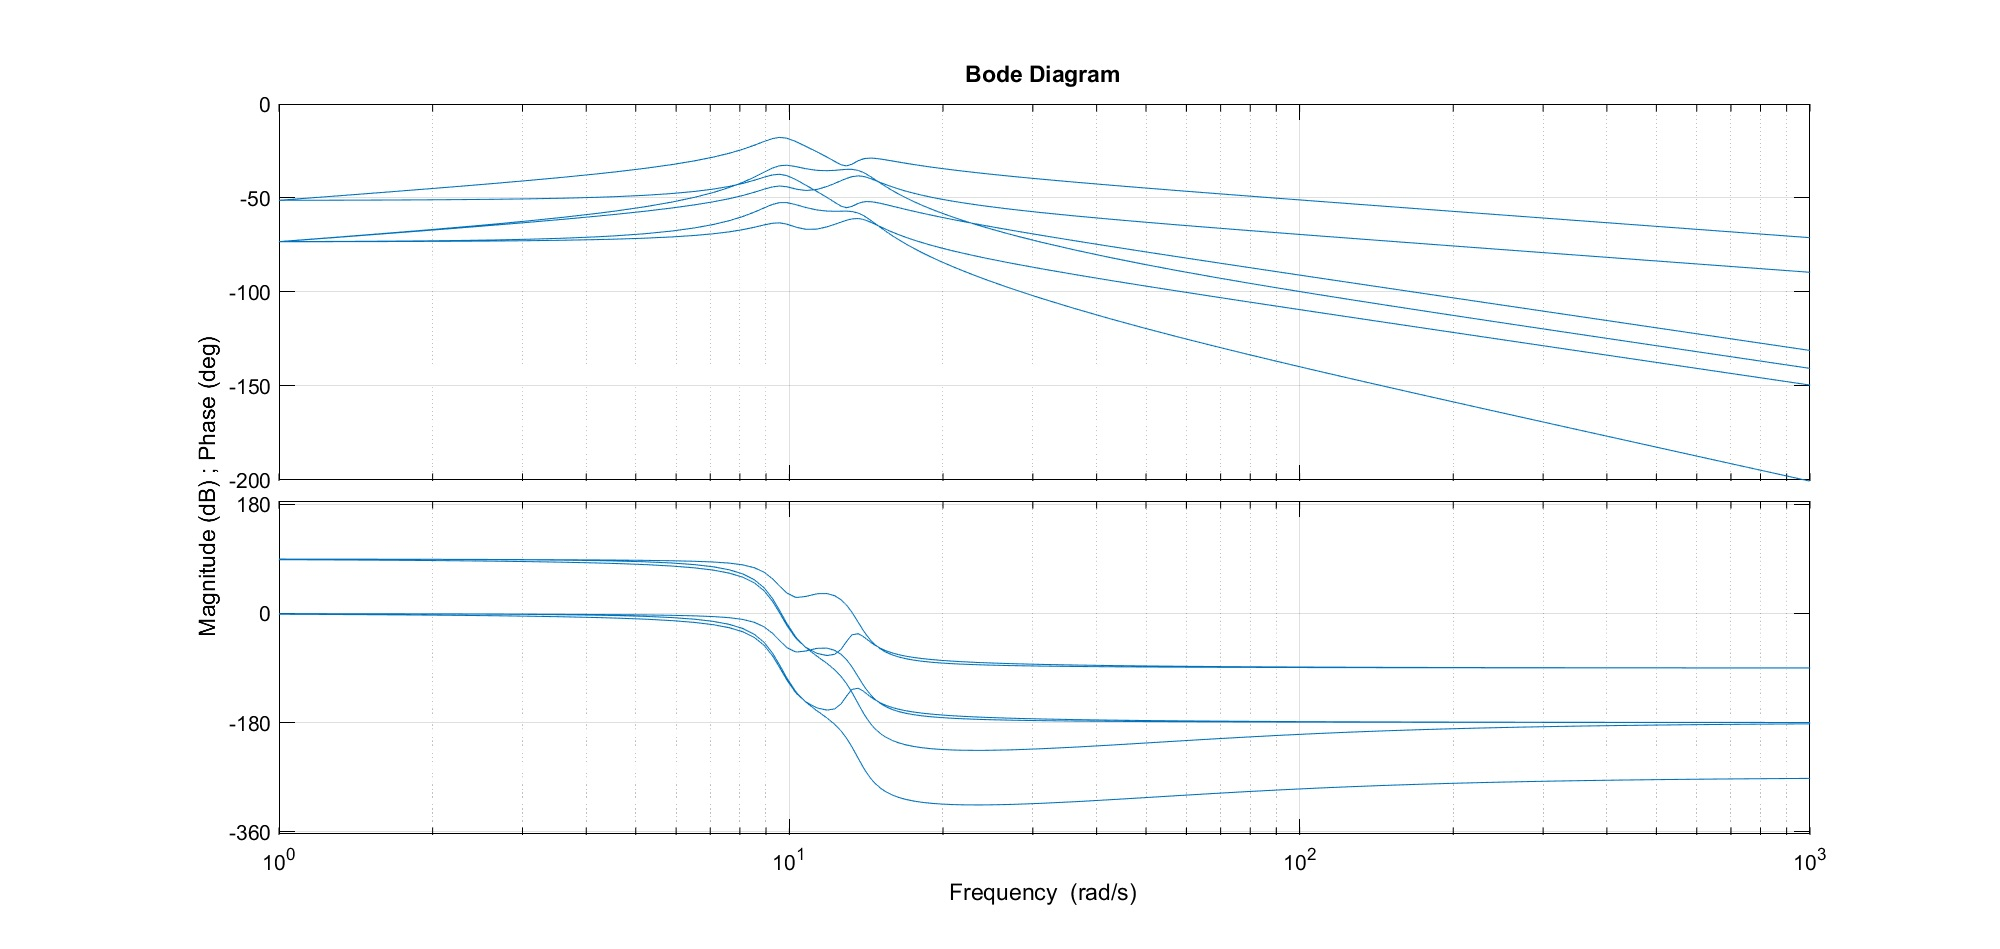
\includegraphics[width=0.7\linewidth]{bode30}
		\caption{Bode plot}
		\label{fig:bode30}
	\end{figure}
	Но частоты определялись по Singular Value Plot, так как работать с Bode Plot в такой формк не удобно.
	\section*{SSP Matlab}
	Для создания и анализа пространства состояний в Matlab, помимо задания переменных были выполнены следующие команды:
	\lstset{frameround=fttt}
	\begin{lstlisting}[firstnumber=1, frame=trBL, firstnumber=1,label=some-code,caption=Создание и анализ SSP в Matlab]
	Sb = ss(A, B, C,D);	%Создание SSP-объекта
	step(Sb);		%Step-response plot
	impulse(Sb);		%Impulse-response plot
	bode(Sb);		%Bode plot
	nyquist(Sb);		%Годограф Найквиста
	K1_2 = damp(Sb);	%Собственные частоты
	\end{lstlisting}

	График реакции на Step-воздействие:
	\begin{figure}[H]
		\centering
		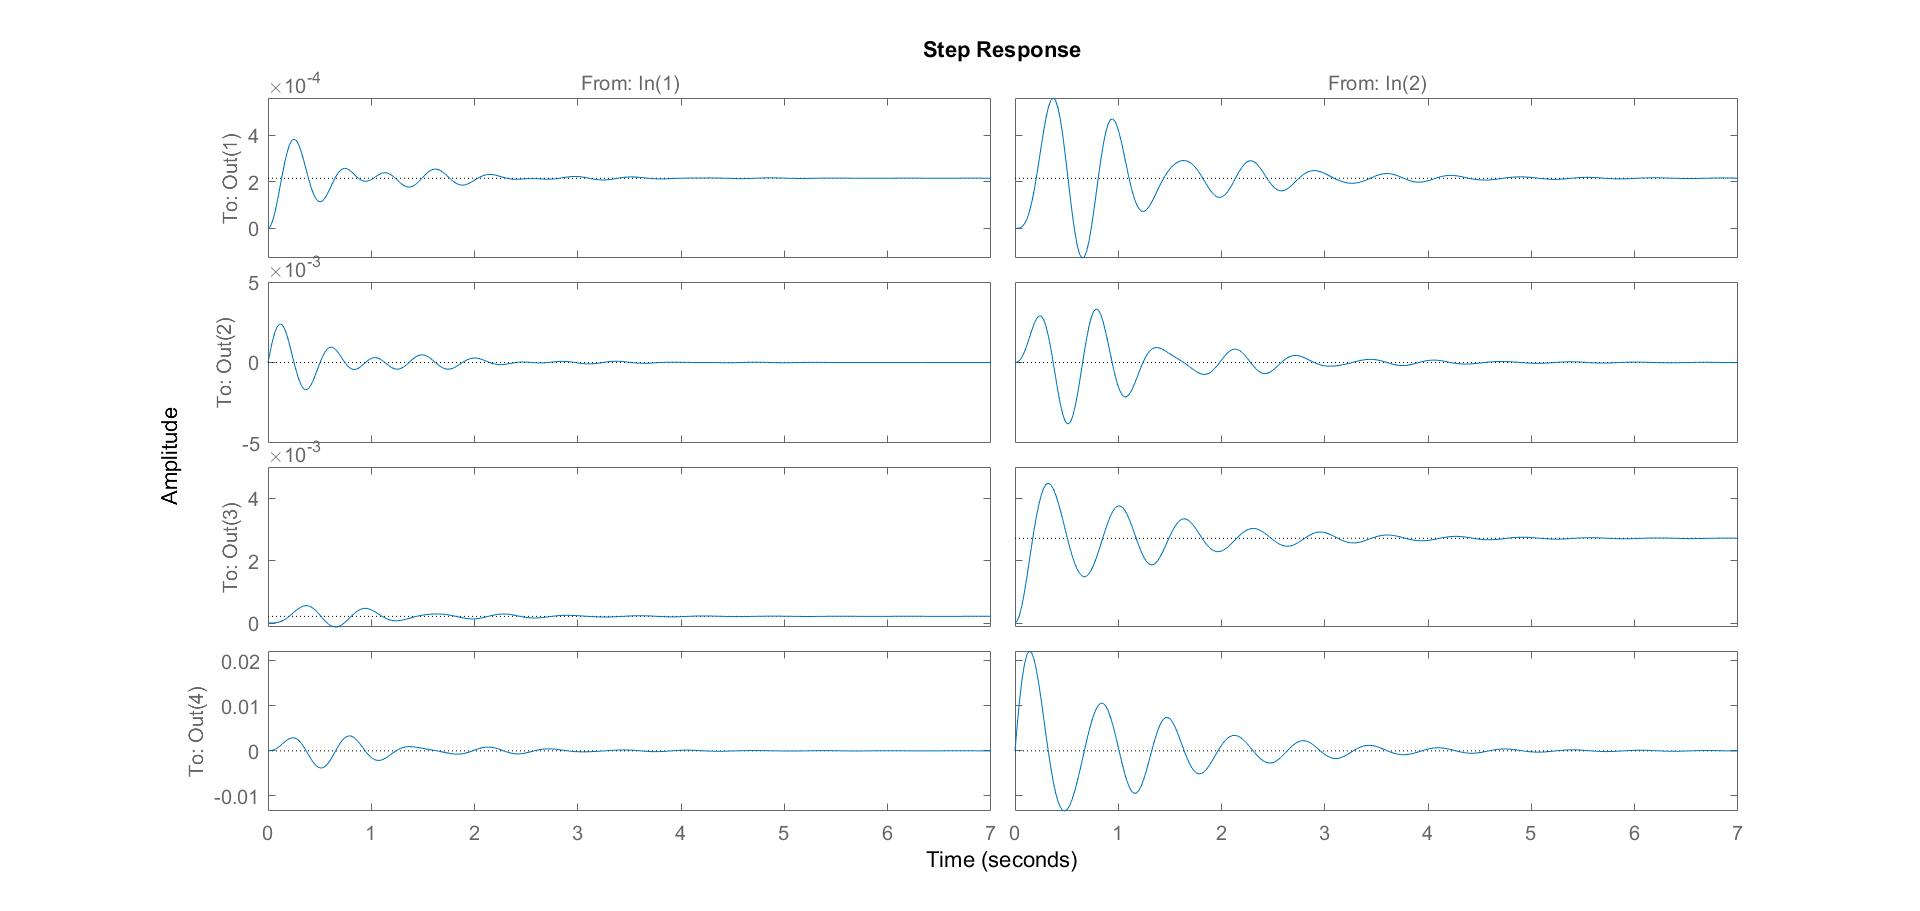
\includegraphics[width=1.2\linewidth]{mstep}
		\caption{Step-response plot}
		\label{fig:mstep}
	\end{figure}
	В отличие от графика, полученного с использованием Simulink, график из Matlab имеет 8 частей. Это связано с тем, что в модели мы имеем два входных параметра (силы) и четыре выходных параметра (скорости и ускорения). Matlab выводит графики влияния каждого из входных параметров на каждый из выходных параметров.
	\begin{figure}[H]
		\centering
		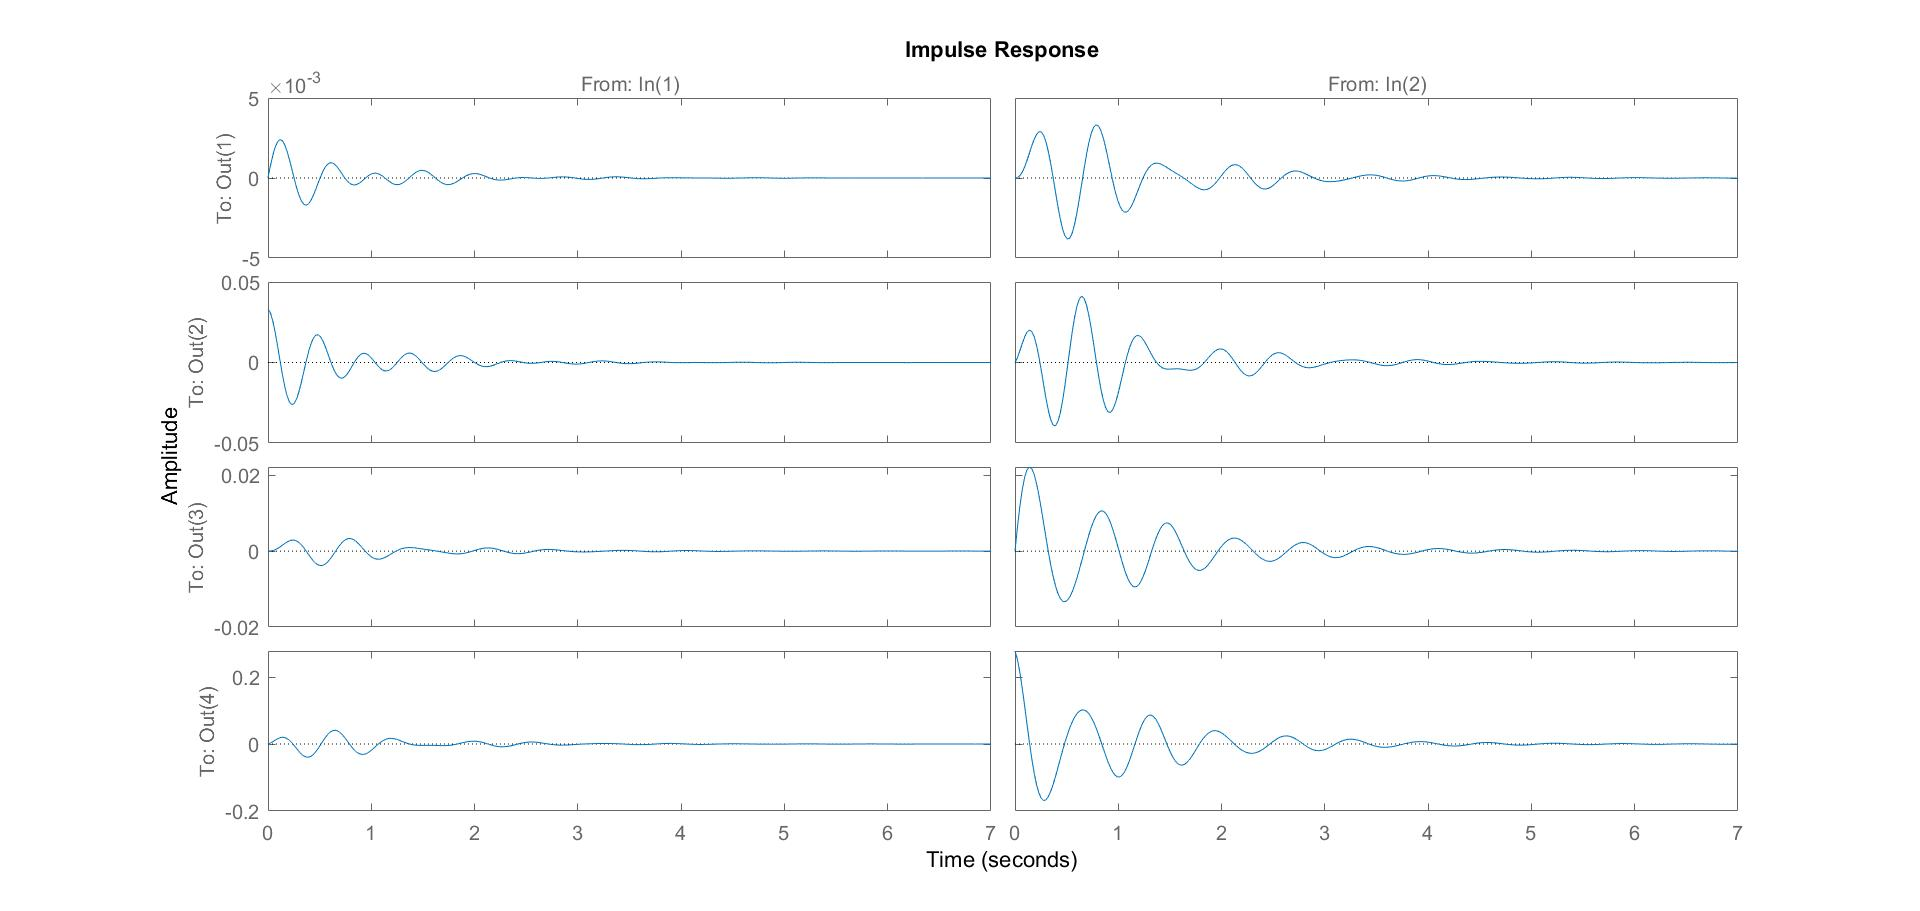
\includegraphics[width=1.2\linewidth]{mimp}
		\caption{График влияния на импульсное воздействие}
		\label{fig:mimp}
	\end{figure}
	Impulse response plot также имеет 8 подграфиков с влиянием каждого параметра на каждый.
	\begin{figure}[H]
		\centering
		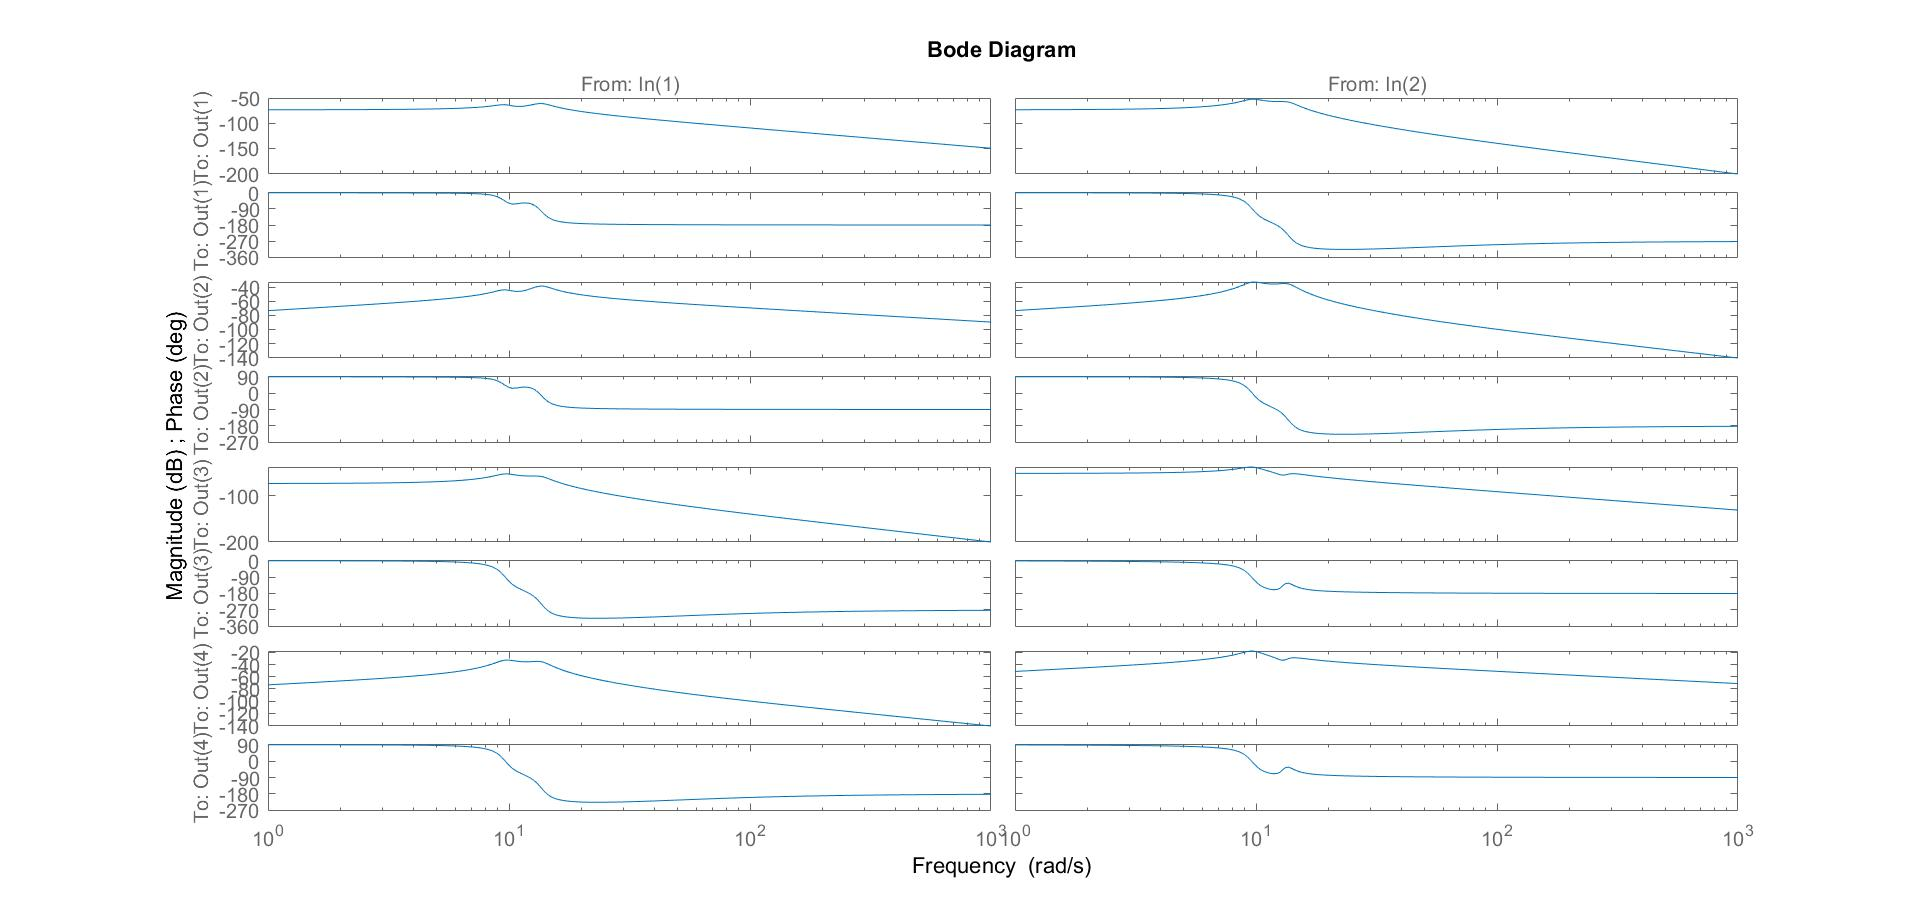
\includegraphics[width=1.2\linewidth]{mbode}
		\caption{Диаграмма Боде}
		\label{fig:mbode}
	\end{figure}
	Диаграмма Боде имеет уже 16 составляющих, так как на каждый параметр приходится по два подграфика: АЧХ и ФЧХ.
	\begin{figure}[H]
		\centering
		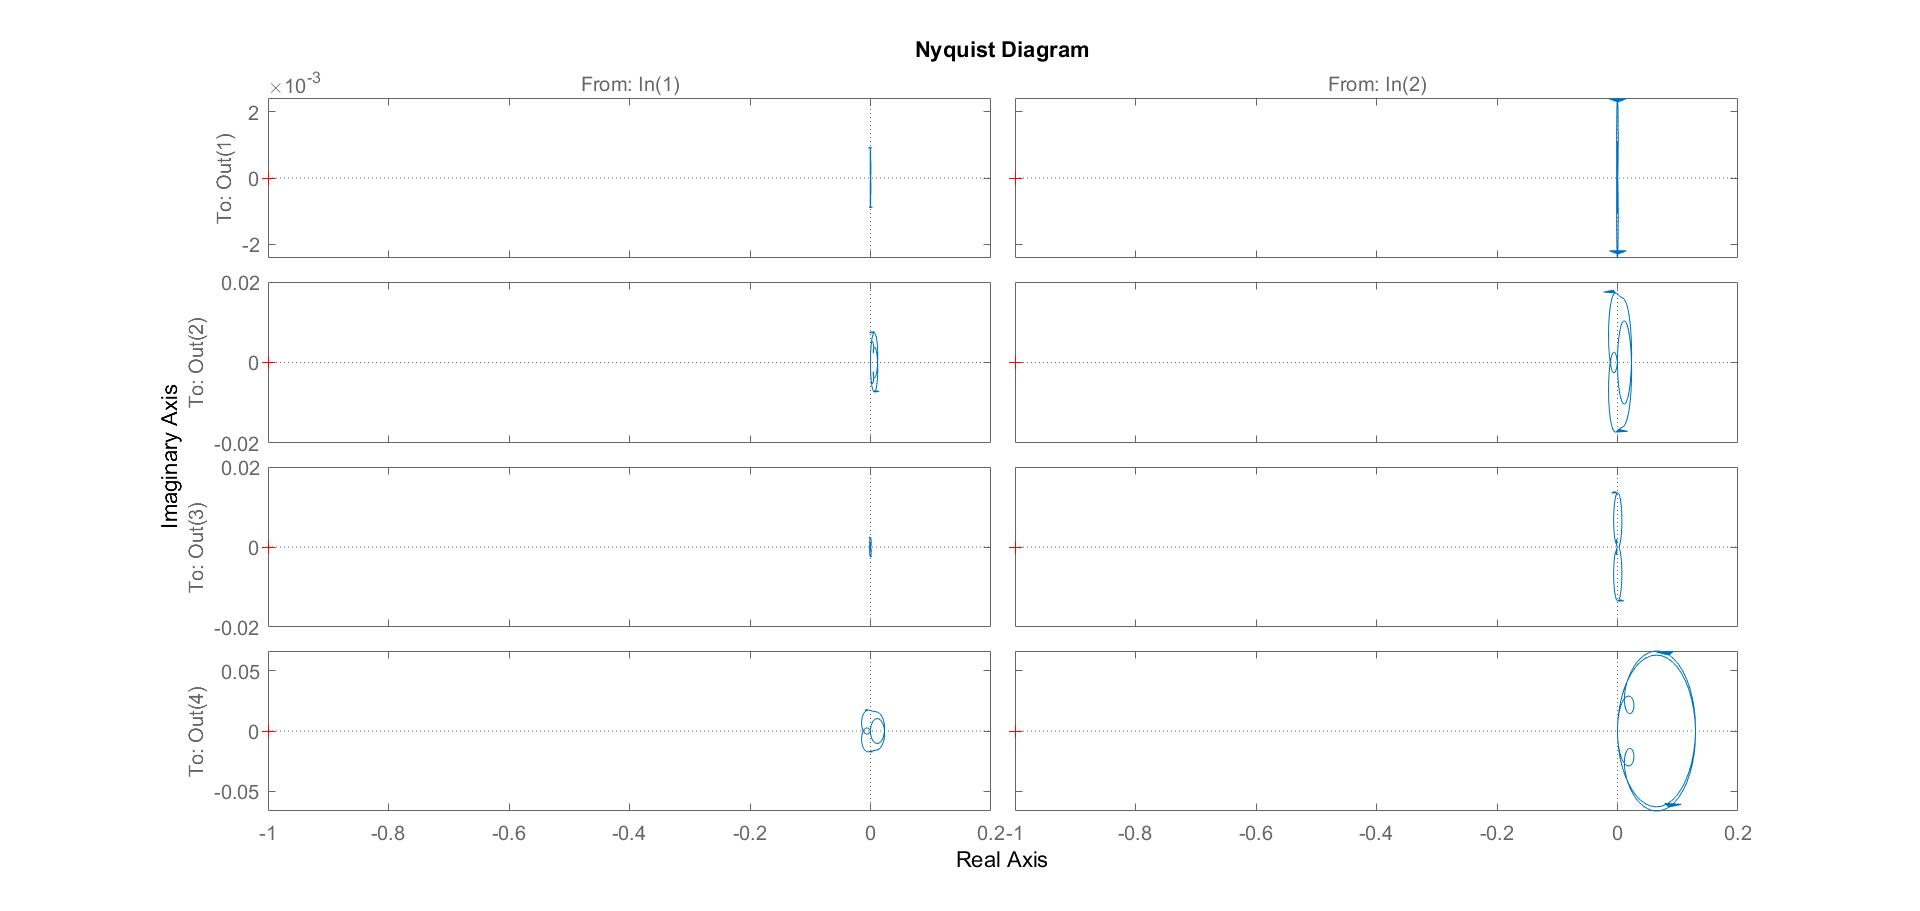
\includegraphics[width=1.2\linewidth]{nyquist}
		\caption{Диаграмма Найквиста}
		\label{fig:nyquist}
	\end{figure}
	Годограф Найквиста показывает устойчивость системы. Так как никакой из параметров не охватывает на комплексной плоскости точку (-1, 0*i), то система устойчива, то есть колебаний не могут начаться самопроизвольно.\\
	Собственные частоты были получены с помощью команды $damp()$. Результат выполнения команды:
	$$k_1 = 9.6479,\ k_2 = 13.6022$$
	Как видно, собственные частоты, полученные в Matlab, вычислены более точно. По крайней мере, расхождение с частотами, полученными в Simulink, начинается с тысячных. Это может быть связано с погрешностями определения частот по графику.
\end{document}